\newpage

\section{Question}
\standards{
  \standard{operators}
}

\begin{itemize}

  \item Show the output of the following program:
    \evaluateCodeLeft{operators-1}{all}
    \vspace{3ex}

  \item Evaluate the following statement piece by piece, using the method shown
    in class (if you are unsure of how this should look, please ask).  If any
    portion of this statement would produce a runtime error (e.g.~by dividing
    by \mintinline{cpp}{0}) stop evaluating at that point, and explain.

    \vspace{2ex}
    \mintinline[fontsize=\Large]{cpp}{1 + 1 - 1 / 1 * + 1 - - - 1 && 1 == ! 1 || 1 + 1 >= 1 / 1 % 1}
    \textAnswer{\par
      \vspace{-1.9em}
      \hspace{-1.2ex}
      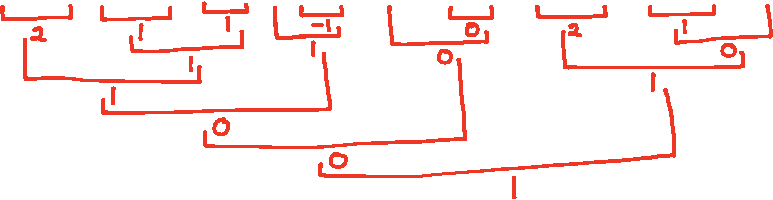
\includegraphics[width=6.37in]{\docImageDir/operators-1}
    }
    \vfill

\end{itemize}

\newpage

